\chapter{Phương pháp tìm hiểu}
\label{Chapter3}

\noindent\textit{Chương này nhóm chúng em trình bày về những đóng góp của bài báo mà nhóm chúng em tìm hiểu được. Ở đây, nhóm chúng em tập trung vào việc xử lý vấn đề thiên lệch dữ liệu, bằng cách sử dụng độ đo khắc phục thiên lệch IPS trong quá trình đánh giá và huấn luyện mô hình. Sau đó, nhóm chúng em trình bày về ``Self Normalized Inverse Propensity Scoring'' (SNIPS) và so sánh với IPS để thấy được sự kết nối giữa IPS và SNIPS cũng như là những điểm lợi và hại của IPS so với SNIPS. Ngoài ra, nhóm chúng em còn trình bày về phương pháp ước lượng ma trận để phục vụ cho việc tính toán độ đo IPS và SNIPS.}

\section{Xem hệ thống gợi ý như một điều trị}
Phần này giới thiệu về phương pháp giải quyết 
Như đã trình bày ở ví dụ về thiên lệch dữ liệu, ta có thể thấy rằng ta chỉ đang quan sát được một phần của dữ liệu mà không thể thấy được toàn bộ sự thật, điều này bị ảnh hưởng bởi rất nhiều yếu tố tiềm ẩn. Giống như việc khi ta muốn xem xét một loại thuốc hay một phương pháp điều trị nhất định có hiệu quả như thể nào đối với bệnh nhân,  giả sử ta tiến hành thử nghiệm phương pháp điều trị đó trên một nhóm bệnh nhân, sau đó ta theo dõi tình trạng bệnh của các bệnh nhân đó, và ta quan sát được sức khỏe của bệnh nhân có chuyển biến tích cực, liệu ta có thể kết luận được rằng phương pháp điều trị đó có thật sự hiệu quả không? Nếu xem xét kĩ lưỡng, có thể rằng phương pháp điều trị của ta có lẽ  khá đắt tiền nên chỉ những người có điều kiện kinh tế ổn định mới có xu hướng dễ tiếp xúc với phương pháp điều trị đó. Mà những người như vậy thì sẽ nhiều điều kiện thuận lợi để chăm sóc sức khỏe bản thân hơn, dẫn đến việc tình trạng bệnh của họ có chuyển biến tích cực hơn. Do đó viêc kiểm tra được độ hiệu quả một phương pháp điều trị không hề đơn giản, người ta thường sử dụng các mô hình nhân quả. Nếu ta xem mỗi người dùng như một bệnh nhân, mỗi bộ phim ta gợị ý giống như một phương pháp điều trị hoặc một loại thuốc, ta sẽ quan tâm đến việc người dùng có phù hợp với bộ phim mà ta gợi ý hay không, phim được gợi ý có khiến người dùng thích thú hay không. Từ đó ta có thể thấy bài toán gợi ý và bài toán được đưa ra khá tương đồng nhau, do có ta cũng sử dụng ý tưởng giải quyết của các phương pháp nhân quả đối với bài toán xem xét hiệu quả điều trị để gợi ý sản phẩm. 

Trong ví dụ về xem xét hiệu quả của một phương pháp điều trị, ta thấy được rằng ta cần phải kiếm soát cả những biến làm ảnh hưởng đến xu hướng mà bệnh nhân có thể tiếp cận được với điều trị đó để mô hình trở nên chính xác hơn, ví dụ như những đặc trưng về nhân khẩu học, thu nhập, mức sống, vị trí sống,... Tuy nhiên sẽ có rất nhiều biến ẩn như vậy mà ta khó có thể kiểm soát  được. Do đó phương pháp nghịch đảo điểm xu hướng ra đời (Inverse propensity scoring - IPS) với ý tưởng rằng ta không cần phải kiếm soát trực tiếp những biến ẩn, mà chỉ cần kiếm soát được xu hướng nhận được điều trị của những bệnh nhân. 

Trong bài toán gợi ý, với giả định rằng người dùng có thể đánh giá hoặc không đánh giá một phim mà họ đã xem, một đánh giá của người dùng dành cho một sản phẩm có thể xuất hiện hoặc không xuất hiện trong tập dữ liệu mà ta qua sát được. Ta có thể biểu diễn điều này thông qua ma trận quan sát O, trong đó các giá trị $O_{u,i}=1$ tương ứng với đánh giá cho bộ phim i từ người dùng u được cung cấp tới hệ thống. Ta đặt $P_{u,i}$ là xác suất mà đánh giá $Y_{u,i}$ có thể quan sát được, hay  $P_{u,i} = P(O_{u,i} = 1)$.  $P_{u,i}$ được gọi là điểm xu hướng của đánh giá  $Y_{u,i}$. Từ các đặc trưng mà ta đã quan sát được về các người dùng, các bộ phim và ma trận quan sát O, ta có thể dự đoán được điểm xu hướng của ma trận đánh giá Y. Phương pháp này sẽ được giới thiệu ở phần tiếp theo của khóa luận này.


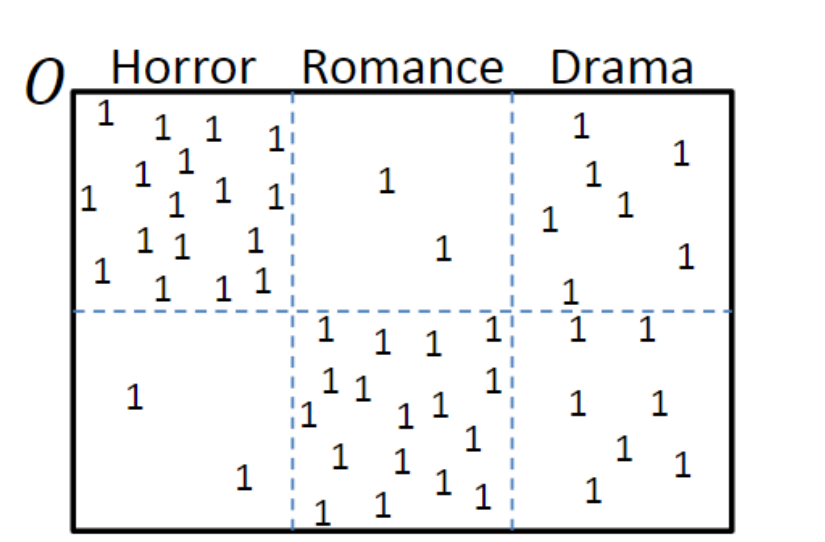
\includegraphics[width=\textwidth]{images/Chapter3/O.png}


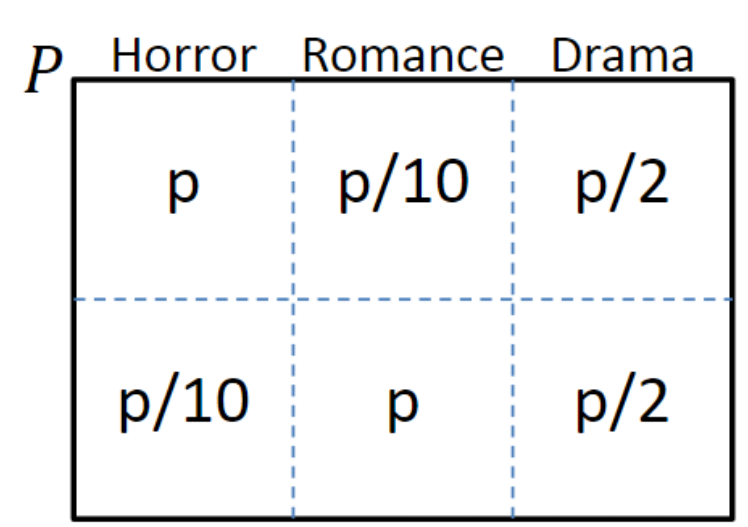
\includegraphics[width=\textwidth]{images/Chapter3/P.png}


Hình ảnh trên minh họa về việc biểu diễn ma trận quan sát O và ma trận xu hướng P. Trong ma trận quan sát O các vị trí có giá trị là 1 đại diện cho đánh giá của người dùng với sản phẩm xuất hiện trong hệ thống, ma trận xu hướng P chứa xu hướng của các đánh giá tương ứng với khả năng ta quan sát được các đánh giá, những phim có số lượt đánh giá nhiều sẽ có điểm xu hướng cao.

\section{``Inverse propensity scoring'' (IPS)}

Nhắc lại về phương pháp tính độ lỗi mà ta thường sử dụng, ta  ký hiệu ma trận đánh giá mà ta quan sát được là Y, ma trận đánh giá mà ta cần phải dự đoán là $\hat{Y}$. Cụ thể, Y là ma trận đánh giá với các đánh giá bị thiếu, $\hat{Y}$ là ma trận đánh giá sau khi được điền đầy đủ các đánh giá bị thiếu. Đầu tiên, mục tiêu của ta là đi tìm một hàm tính độ lỗi của $\hat{Y}$ so với Y mà phản ánh được độ lỗi thật sự chỉ bằng tập dữ liệu quan sát được Y. Thông thường, hàm tính độ lỗi sẽ được biểu diễn như sau:
\begin{equation}
\label{eq:tradition}
R(\hat{Y}) = \frac{1}{U\cdot I}  \sum_{u=1}^{U} \sum_{i=1}^{I} \delta_{u,i}(Y,\hat{Y})
\end{equation}

Trong đó, $\delta$ là một hàm tính độ lỗi bất kì
Nhưng vì ta chỉ có thể quan sát được một phần của toàn bộ đánh giá, do đó ta chỉ tính trung bình độ lỗi của các đánh giá quan sát được, ta tạm gọi hàm lỗi này là hàm lỗi ngây thơ(Naive), hàm lỗi này có công thức như sau:
\begin{equation}
\label{eq:naive}
R_{Naive}(\hat{Y}) = \frac{1}{|\{(u,i):O_{u,i} = 1\}|} \sum_{(u,i):O_{u,i}=1}^{I} \delta_{u,i}(Y,\hat{Y}) 
\end{equation}
Sự ngây thơ của hàm lỗi này đã dấn đến việc đánh giá mô hình bị sai ở ví dụ về thiên lệch lựa chọn trong phần giới thiệu. Do mẫu dữ liệu mà ta quan sát được không được phát sinh ngẫu nhiên theo phân phối đều từ dữ liệu thực tế mà bị tác động bởi thiên lệch lựa chọn. Đó là lý do tại sao hàm lỗi ngây thơ lại có giá trị khác biệt so với độ lỗi thực tế, người ta gọi đây là một hàm lỗi bị lệch (bias), hay nói cách khác, kỳ vọng của hàm lỗi này khác với độ lỗi thực tế.
\[E_O [R_{Naive} (\hat{Y})] \ne R(\hat{Y})\]

Hiểu được vấn đề của hàm lỗi ngây thơ, tác giả đưa ra một hàm lỗi thay thế giúp giải quyết được vấn đề dữ liệu bị lệch.Phương pháp dựa trên một phương pháp thường được sử dụng trong các mô hình nhân quả, gọi là phương pháp nghịch đảo điểm xu hướng. Trong phạm vi của bài báo mà nhóm em tìm hiẻu, tác giả tiến hành hai loại nghiên cứu là nghiên cứu quan sát và nghiên cứu thực nghiệm:
\begin{itemize}
    \item Nghiên cứu thực nghiệm: trong nghiên cứu này, ta có thể điều khiển hệ thống gợi ý của ta bằng cách quyết định những sản phẩm nào sẽ được hiển thị đến người dùng, từ đó ta có thể biết được điểm xu hướng của nó.
    \item Nghiên cứu quan sát: trong nghiên cứu này, ta sẽ thu thập dữ liệu có sẵn từ một hệ thống đánh giá phim có sẵn, trong hệ thống này người dùng có quyền tự chọn những bộ phim họ xem và đánh giá. Do đó, ta không biết được điểm xu hướng mà cần phải tiến hành ước lượng nó. Phương pháp ước lượng này sẽ được trình bài cụ thể trong phần 3.3 thông qua các mô hình như Naive Bayes và Logistic Regression.
\end{itemize}

Áp dụng nghịch đảo điểm xu hướng đã được nghiên cứu bởi Little và Rubin 2000; Thompson, 2012; Imbens và Rubin, 2015 để sử dụng cho hàm lỗi của hệ thống gợi ý, ta định nghĩa công thức tính độ lỗi IPS như sau:
\begin{equation}
\label{eq:IPS}
R_{IPS}(\hat{Y}|P) = \frac{1}{U\cdot I}\sum_{(u,i):O_{u,i}=1} \frac{\delta_{u,i}(Y,\hat{Y})}{P_{u,i}}
\end{equation}

Về cơ bản, điểm xu hướng này luôn luôn lớn hơn 0 ở mọi cặp người dùng - sản phẩm để chắc chắn mỗi phần tử trong ma trận đánh giá Y đều có thể được quan sát và tổng nghịch đảo các điểm xu hướng của các đánh giá mà ta quan sát được sẽ bằng với số lượng đánh giá của toàn bộ người dùng dành cho toàn bộ sản phẩm hay:

\begin{equation}
\label{eq:EO}
E_O\bigg[\sum_{(u,i):O_{u,i}=1} \frac{1}{P_{u,i}}\bigg] = U \cdot I
\end{equation}

\begin{lemma}
(Sự không thiên lệch của IPS)
Với mọi người dùng u và sản phẩm i, nếu điểm xu hướng $P_{u,i} \in (0,1)\text{ và }  P_{u,i}>0, \text{ thì }  R_{IPS}(\hat{Y}|P)$ là một độ đo không thiên lệch của $R(\hat{Y})$, có nghĩa là kì vọng của $R_{IPS}(\hat{Y}|P)$ bằng với $R(\hat{Y})$
\end{lemma}

\textit{Chứng minh.} 
\begin{equation}
\begin{aligned}
\mathcal\mathbb{E}_{O} \Bigg[R_{IPS}(\hat{Y}|P)\Bigg] &=  \frac{1}{U\cdot I} \cdot \sum_{u=1}^{U} \sum_{i=1}^{I} \mathbb{E}_{O} \Bigg[ \frac{\delta_{u,i}(Y,\hat{Y}}{P_{u,i}}{O_{u,i}}\Bigg] \\ &= \frac{1}{U\cdot I} \cdot \sum_{u=1}^{U} \sum_{i=1}^{I}\delta_{u,i} \\ &
= R(\hat{Y})
\end{aligned}
\end{equation}

\section{``Self normalized inverse propensity scoring'' (SNIPS)}


\begin{equation}
\label{eq:snips}
\hat{R}_{SNIPS}(\hat{Y}|P) = \frac{\frac{1}{U \cdot I}\sum_{(u,i):O_{u,i}=1} \frac{ \delta_{u,i} (Y,\hat{Y}}{P_{u,i}})}{\sum_{(u,i):O_{u,i}=1} \frac{1}{P_{u,i}}} U \cdot I = \frac{\sum_{(u,i):O_{u,i}=1} \frac{ \delta_{u,i} (Y,\hat{Y}}{P_{u,i}})}{\sum_{(u,i):O_{u,i}=1} \frac{1}{P_{u,i}}}
\end{equation}

\section{Ước lượng ma trận xu hướng}
Trước tiên, để hiểu được các phương pháp ước lượng xu hướng của một đánh giá hay nói các khác là khả năng mà một đánh giá được quan sát, ta cần hiểu được các loại mất mát dữ liệu. Đầu tiêu là MAR (Mising At Random), có nghĩa là sự mất mát dữ liệu này là ngẫu nhiên. Kiểu mất mát này là kiểu ta thường giả định trong học máy. Ở kiểu mất mát này, ta có thể ước lượng được giá trị bị thiếu thông qua các giá trị quan sát được. Ví dụ như trong nghiên cứu về thông tin nhân khẩu học, nếu ta giả định rằng giá trị thu nhập bị thiếu là ngẫu nhiên thì ta có thể ước lượng thu nhập bị thiếu dựa vào các thông tin ta quan sát được như độ tuổi, nghề nghiệp, nơi sống,..Tuy nhiên,  một kiểu mất mát dữ liệu khác là MNAR (Missing Not At Random), ở kiểu mất mát này ta sẽ khó ước lượng được thu nhập bị thiếu vì các giá trị bị thiếu thường có một nguyên nhân nào đó, và nó mang một ý nghĩa nhất đinh. Trong trường hợp trên, có thể những người dùng có thu nhập cao có xu hướng hạn chế công khai thu nhập của bản thân, do đó những thu nhập bị thiếu có thể cao hơn phần thu nhập ta quan sát được rất nhiều do đó không thể ước lượng bằng các mô hình học máy thông thường. Còn một kiểu mất mát khác là MCAR (Missing Completely At Random), có nghĩa là sự mất mát dữ liệu là hoàn toàn ngẫu nhiên, các mẫu mà ta quan sát được có thể xem như những mẫu đại diện, do đó ta có thể xóa những mẫu có dữ liệu bị thiếu. Ta có thể tìm hiểu kĩ hơn về các vấn đề mất mát dữ liệu trong nghiên cứu của Little và Rubin, 2002.
Xét nghiên cứu quan sát trêntrên tập dữ liệu ML100K được cung cấp bởi Grouplens, ta dễ thấy các đánh giá bị thiếu không phải do ngẫu nhiên (MNAR) mà do thiên lệch lựa chọn của người dùng và của hệ thống gợi ý đã sử dụng. Do đó ta không biết được xu hướng của các đánh giá mà  cần ước lượng xu hướng $P_{u,i}$ của mỗi đánh giá của người dùng u dành cho sản phẩm i sẽ được quan sát. Nói chung, xác suất một đánh giá ta có thể quan sát được có thể phụ thuộc vào các đặc trưng có thể quan sát được X (ví dụ như điểm số đánh giá dự đoán được hiển thị cho người dùng), các đặc trưng không thể quan sát được $X^{hid}$ (ví dụ như sản phẩm đó có được giới thiệu bởi bạn bè của người dùng hay không), và đánh giá Y:

\begin{equation}
\label{eq:pui}
    P_{u,i}=P(O_{u,i} = 1|X, X^{hid},Y)
\end{equation}
Do đó khi các đặc trưng có thể quan sát được đã được sử dụng để tính toán, ta có cơ sở để giả định rằng $O_{u,i}$ độc lập với ma trận dự đoán mới $\hat{Y}$ nên nó độc lập với $\delta_{u,i}(Y,\hat{Y})$. Như đã đề cập ở trên, ta sử dụng hai phương pháp đơn giản để ước lượng ma trận xu hướng.

\subsection{Ước lượng ma trận xu hướng thông qua Naive bayes}

Để thực hiện được phương pháp Naive Bayes cho ước lượng ma trận xu hướng, ta cần phải giả định rắng sự phụ thuộc giữa các biến X,   $X_{hid}$ và các đánh giá khác là không đáng kể. Do đó công thức \ref{eq:pui} được đơn giản thành $P(O_{u,i}|Y_{u,i})$ tương tự như Marlin và Zemel (2009). Ta có thể xem $Y_{u,i}$ như là những mẫu đánh giá mà ta quan sát được, khi đó ta chỉ cần ước lượng các điểm xu hướng cho những đánh giá quan sát được để tính toán IPS và SNIPS. Ta sử dụng Naive Bayes để ước lượng các xu hướng này như sau:
\begin{equation}
\label{eq:pnb}
    P(O_{u,i} = 1| Y_{u,i} = r) = \frac{P(Y=r|O=1)P(O=1)}{P(Y=r)}
\end{equation}
Trong đó việc ước lượng hợp lý cực đại cho $P(Y=r|O=1)$ và $P(O=1)$ có thể được tính toán thông qua đếm số đánh giá  quan sát được trong dữ liệu MNAR. Tuy nhiên, khi muốn ước lượng $P(Y=r) = P(Y=r|O=1) + P(Y=r|O=0)$, ta cần phải có một mẫu nhỏ MCAR. Phương pháp cụ thể để tìm tập nhỏ MNAR sẽ được trình bày ở phần thực nghiệm.  

\subsection{Ước lượng ma trận xu hướng thông qua Logistic regression}
Một hướng tiếp cận khác để giải quyết việc  ước lượng ma trận xu hướng là sử dụng hồi quy Logistic. Phương pháp này có ưu điểm là không yêu cầu một tập mẫu nhỏ MCAR. Cũng dựa trên công thức \ref{eq:pui}, nhưng mục tiêu của ta là tìm một bộ tham số $\phi$ sao cho ma trận quan sát O có thể độc lập với ma trận ma
trận đặc trưng không quan sát được $X^{hid}$ và Y. Nói cách khác, $P(O_{u,i} = 1|X, X^{hid},Y) = P(O_{u,i}|X,\phi)$. Ở phương pháp này, ta giả định rằng tồn tại một bộ tham số $\phi=(\omega, \beta, \gamma)$ sao cho
\begin{equation}
    \label{eq:plr}
    P_{u,i} = \sigma(\omega^TX_{u,i} + \beta_i + \gamma_u)
\end{equation}
Trong đó, $X_{u,i}$ là vector được vector hóa từ những thông tin quan sát được về các cặp người dùng, sản phẩm (ví dụ như thông tin nhân khẩu học của người dùng, bộ phim có được quảng cáo hay không), $\sigma(\cdot)$ là hàm sigmoid, $\beta_i, \gamma_u$ là phần per-item và per-user

\section{Phân rã ma trận kết hợp với IPS}
Ở phần trước, ta đã tìm hiểu về phương pháp IPS và cải tiến của nó giúp giảm phương sai cho mô hình gọi là SNIPS, ngoài ra ta còn tìm hiểu về cách ước lượng xu hướng của các đánh giá hay còn gọi là xác suất để các đánh giá xuất hiện trong tập dữ liệu mà ta quan sát được. Trong phần này, dựa vào những kiến thức đã trình bày trước đó, nhóm em sẽ sử dụng hàm lỗi mới để phân rã ma trận dựa trên công thức \ref{eq:IPS}. 

Phát biểu bài toán: Với ma trận quan sát O, ma trận đánh giá Y, ma trận xu hướng P, không gian giả thuyết $\mathcal{H}$ của các dự đoán $\hat{Y}$ và hàm lỗi $\delta_{u,i}(Y, \hat{Y})$. Mục tiêu của ta là tìm $\hat{Y}$ sao cho:
\begin{equation}
    \label{eq:ERM}
    \hat{Y} = \underset{\hat{Y} \in \mathcal{H}}{argmin}\bigg\{\hat{R}_{IPS}(\hat{Y}|P\bigg\}
\end{equation}

Tiếp theo, để giải quyết bài toán dự đoán đánh giá $\hat{Y}$, ta sử dụng phương pháp pháp phân rã ma trận (Matrix Factorization) như đã trình bày ở chương trước. Giả sử ta xem mô hình phân rã ma trận với nhiệm vụ dự đoán mỗi đánh giá $\hat{Y}_{u,i} = \upsilon_u^T \omega_i + a_u + b_i + c$ với $a_u$ là  offset tương ứng của từng người dùng, $b_i$ là offset của sản phẩm, c là offset toàn cục của không gian giả thuyết $\mathcal{H}$. Từ đó ta có thể xem mục tiêu huấn luyện của ta là:

\begin{equation}
    \label{eq:objective}
    \underset{V,W,A}{argmin} \bigg[ \sum_{(u,i):O_{u,i}=1} \frac{\delta_{u,i}(Y,V^TW + A)}{P_{u,i}} + \lambda(||V||_{F}^2 + ||W||_{F}^2) \Bigg]
\end{equation}

Với A tương ứng với offset và $\hat{Y} = V^TW + A$ 

Ta có thể thấy rằng, các phương pháp phân rã ma trận truyền thống là một trường hợp đặc biệt của công thức \ref{eq:objective}, với tất cả những xu hướng $P_{u,i}$ đều bằng nhau. Hay nói cách khác, khả năng xuất hiện của các đánh giá là như nhau, điều này xuất phát từ một giả định không chính xác của ngưởi dùng là là dữ liệu đánh giá mà ta thu thập được là MCAR. Đây chính là điểm đặc biệt của mô hình mà nhóm em tìm hiểu. Mô hình này có vẻ không có quá nhiều khác biệt so với các mô hình thông thường được xây dựng trước đó, chỉ khác nhau một phần nhỏ ở hàm mục tiêu. Tuy nhiên, thách thức của việc tìm được ma trận xu hướng P là khá lớn, và khó để tìm chính xác được một ma trận xu hướng P để ta có thể thấy được toàn bộ dữ liệu thật sự dựa vào dữ liệu quan sát được. 